\subsection{Setup Time e Hold Time}

Para que elementos de memória, como flip-flops, que veremos na sessão \textbf{4.4}, operem corretamente, é necessário que suas entradas satisfaçam restrições temporais em relação ao sinal de clock.

\begin{figure}[H]
    \centering
    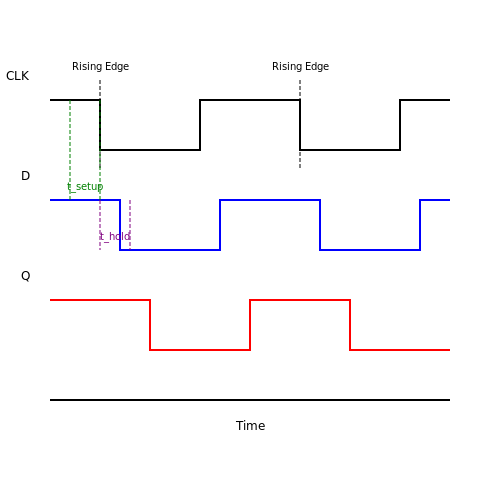
\includegraphics[width=0.7\linewidth]{images/setup-hold-times.png}
    \caption{Exemplo de setup e hold times para um Flip Flop tipo D}
    \label{fig:setup-hold-times}
\end{figure}

O \textit{setup time} ($t_{setup}$) é o intervalo mínimo antes da borda ativa do clock durante o qual a entrada deve permanecer estável.

O \textit{hold time} ($t_{hold}$) é o intervalo mínimo após a borda do clock durante o qual a entrada deve continuar estável.

Formalmente, se $t_0$ representa o instante da borda do clock, a entrada deve permanecer inalterada no intervalo:

\[
[t_0 - t_{setup},\ t_0 + t_{hold}]
\]

A violação dessas restrições pode levar a comportamentos incorretos.